%!TEX root = umthsmpl.tex
\chapter{Location privacy without carrier cooperation}
In this chapter, I present methods for users to achieve cell phone anonymity without requiring trust in the service provider\footnote{This chapter is based in part on work published at the IEEE Workshop on Mobile System Technologies~\cite{sung:2014}}. In the preliminary work, I present a GSM-compatible framework that allows for virtual SIM cards so that a user could change her identity regularly. I also present a simple analysis that shows even such a system is susceptible to location profiling, and may not afford the user the desired privacy.

\section{Preliminary work: Anonymous cell phone systems and vulnerabilities}

% Several products exist to 
In this chapter, I prevent several methods a user may pursue to break the link between herself and the cell phone's identifier on the network (i.e. this is an identifier associated with an electronic serial number on the phone or SIM card). These methods are
fully compatible with deployed GSM protocols and infrastructure, from 2G systems typically deployed in poor regions of the world to the new 4G standards deployed in Europe and the US. In our attacker model, we consider carriers that are at best uncooperative, and at worst active adversaries.

\paragraph*{Methods for anonymous cell phone usage}

The most naive method to achieve location privacy is to \textit{anonymously purchase many burner phones}, and use each of them depending on context. 
% TODO: check if these services exist online already
This comes at a high cost, and limits the amount of identifiers a user may have access to. I propose two additional methods: one is a software-based authentication scheme (\textit{ZipPhone}) that requires the cooperation of a mobile virtual network operator (MVNO) that is privacy proactive; the second is a SIM-sharing scheme (\textit{Spartacus}) that allows users to form mix-zones with other users to swap identities.

I plan to investigate the effectiveness of each of these methods, including ease of use, monetary cost, vulnerabilities, and privacy achieved. 

\paragraph*{ZipPhone}
Using a WiFi connection not observable to the cellular 
carrier, a user bootstraps ZipPhone by paying an MVNO for service using an anonymous electronic 
currency~\cite{Ben-Sasson:2014,Miers:2013,Bissias:2014}. Upon payment, the user receives 
one or more IMSIs. This step delinks users and identifiers. 
The user is now ready to use make and receive calls using VOIP. To do so, 
they connect to the GSM network, authenticating themselves with the IMSI, 
which the MNO will verify via signaling to the MVNO (see~\cite{sung:2014} 
for details).

The user periodically discards IMSIs to avoid the gathering  of 
sufficient geographical information by the carrier to classify successfully against 
known profiles of users.  If the user wishes to purchase additional 
ZipPhone IMSIs, they need not necessarily utilize WiFi again. They can 
use their carrier-provided data connection, and contact the ZipPhone 
MVNO using secure protocols over the Internet to do so.

\paragraph*{Spartacus}
A SIM owner can leave an extra Internet-connected phone at their house or other
preferred location (perhaps with the actual SIM) and instruct it to
connect to the network remotely; this setup allows the owner to
reclaim without necessarily revealing their current location. 
Peers that wish to lend out use of their SIM can retrieve the $K_i$
key stored in it (this is done only once), or do a man-in-the-middle attack between the phone and SIM during each remote authentication. They can then
produce the $K_c$ and SRES values for a remote ZipPhone requester, who
can relay via Wi-Fi (or existing cellular connection) the {\em random number} issued by the carrier to the peer during a location update. Keys 
for encryption with GPRS/EDGE also are based on knowledge of $K_i$ and can be similarly relayed.

\paragraph*{Location profiling}
\begin{figure}
	\centering
	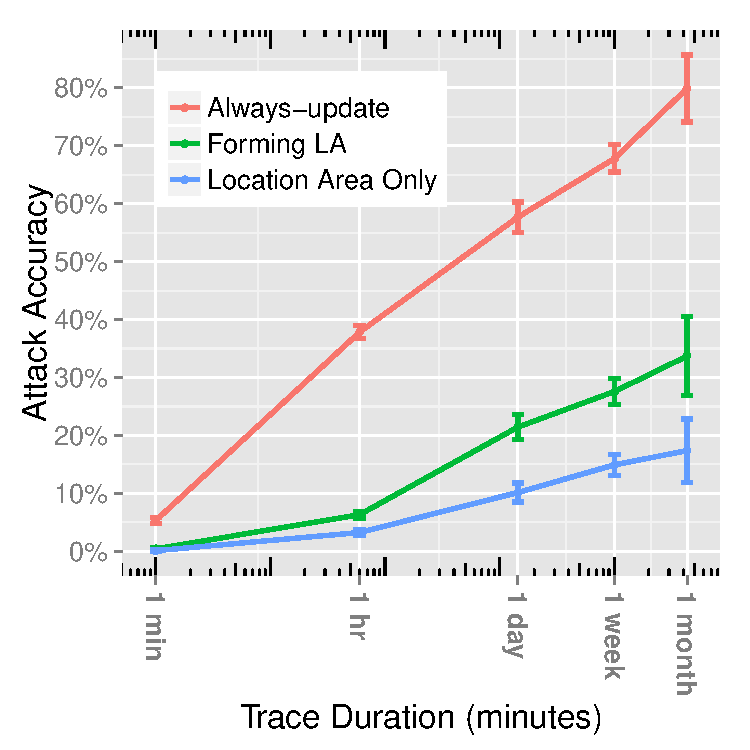
\includegraphics[width=0.7\textwidth]{graphics/mulder}
	\caption{The accuracy of the attack defined by Mulder et al.~\cite{Mulder:2008} under the always-update policy (top, blue line) and forming LA policy (middle, red line). Our results match well with\cite{Mulder:2008}: an attacker achieves a 38\% success rate against users that update their SIM-based identifiers once an hour.  Under the latter, more realistic, forming location area update policy, the attacker's success rate falls to 6\% when SIM-based identifiers are updated once an hour. The bottom, green line shows the lower bound on any scheme: it represents an unrealistic location management scheme where the carrier learns only the location area but not the cell a user is associated with. Errorbars represent 95\% c.i.}
	\label{fig:mulder}
\end{figure}

The effectiveness of the classifier is shown in Figure~
\ref{fig:mulder}. In all cases, the attacker is given a preceding month's 
data as ground truth for training. The blue line is a recreation of results 
from Mulder et al.: a randomly selected  1-month-long sequence of the cells a 
user is associated with results in a high accuracy  of 80\%; Mulder et 
al.\ saw\footnote{These small differences are due to our use of an additional month from the data set.} about 82\%. A random sample of up to 1-hour of cell locations is identifiable 38\% of the time; Mulder et al.\ saw about 44\%. In both cases, random chance would be correct about 1\% of the time. 

% TODO: portknocking
\paragraph*{Fake pages}
In modern GSM networks, phones communicate to specific towers only
when a call (or SMS text or GPRS data packet) is incoming or
originated, rather than whenever a new tower is in
range\cite{Razavi:2011,Wong:2000}. However, a more advanced and
aggressive attacker will proactively cause a phone to communicate with
its nearest tower~\cite{Ficek:2013a} based on an SMS {\em Class 0}
message, ICMP ping, or similar technique.

We can defend against these pages with page-knocking, where the handset answers data pages only after a correct sequence is received (all other pages are ignored). Specifically, the VoIP proxy agree on a  function (e.g., a cryptographic hash) that accepts as input a shared secret key and the current time (in minute granularity). The output of the function is then take one bit at a time: if the bit is zero, no packets are sent (and thus no pages) for $d$ seconds; if the bit is one, a packet (and one page) is sent and then it pauses $d$ seconds. The handset can answer at any time; the proxy doesn't need to know the value $n$. An initial non-empty page is required to start the sequence.

The chances that the carrier can falsify the sequence is $2^{-n}$ for an $n$-bit sequence. The cost is that the user must wait $(n+1)d$ seconds before answering incoming pages for VoIP calls. On Verizon, I have measured $d$ to be $5.12 * 2$ seconds. 

 \begin{figure}[t] 
	\centering{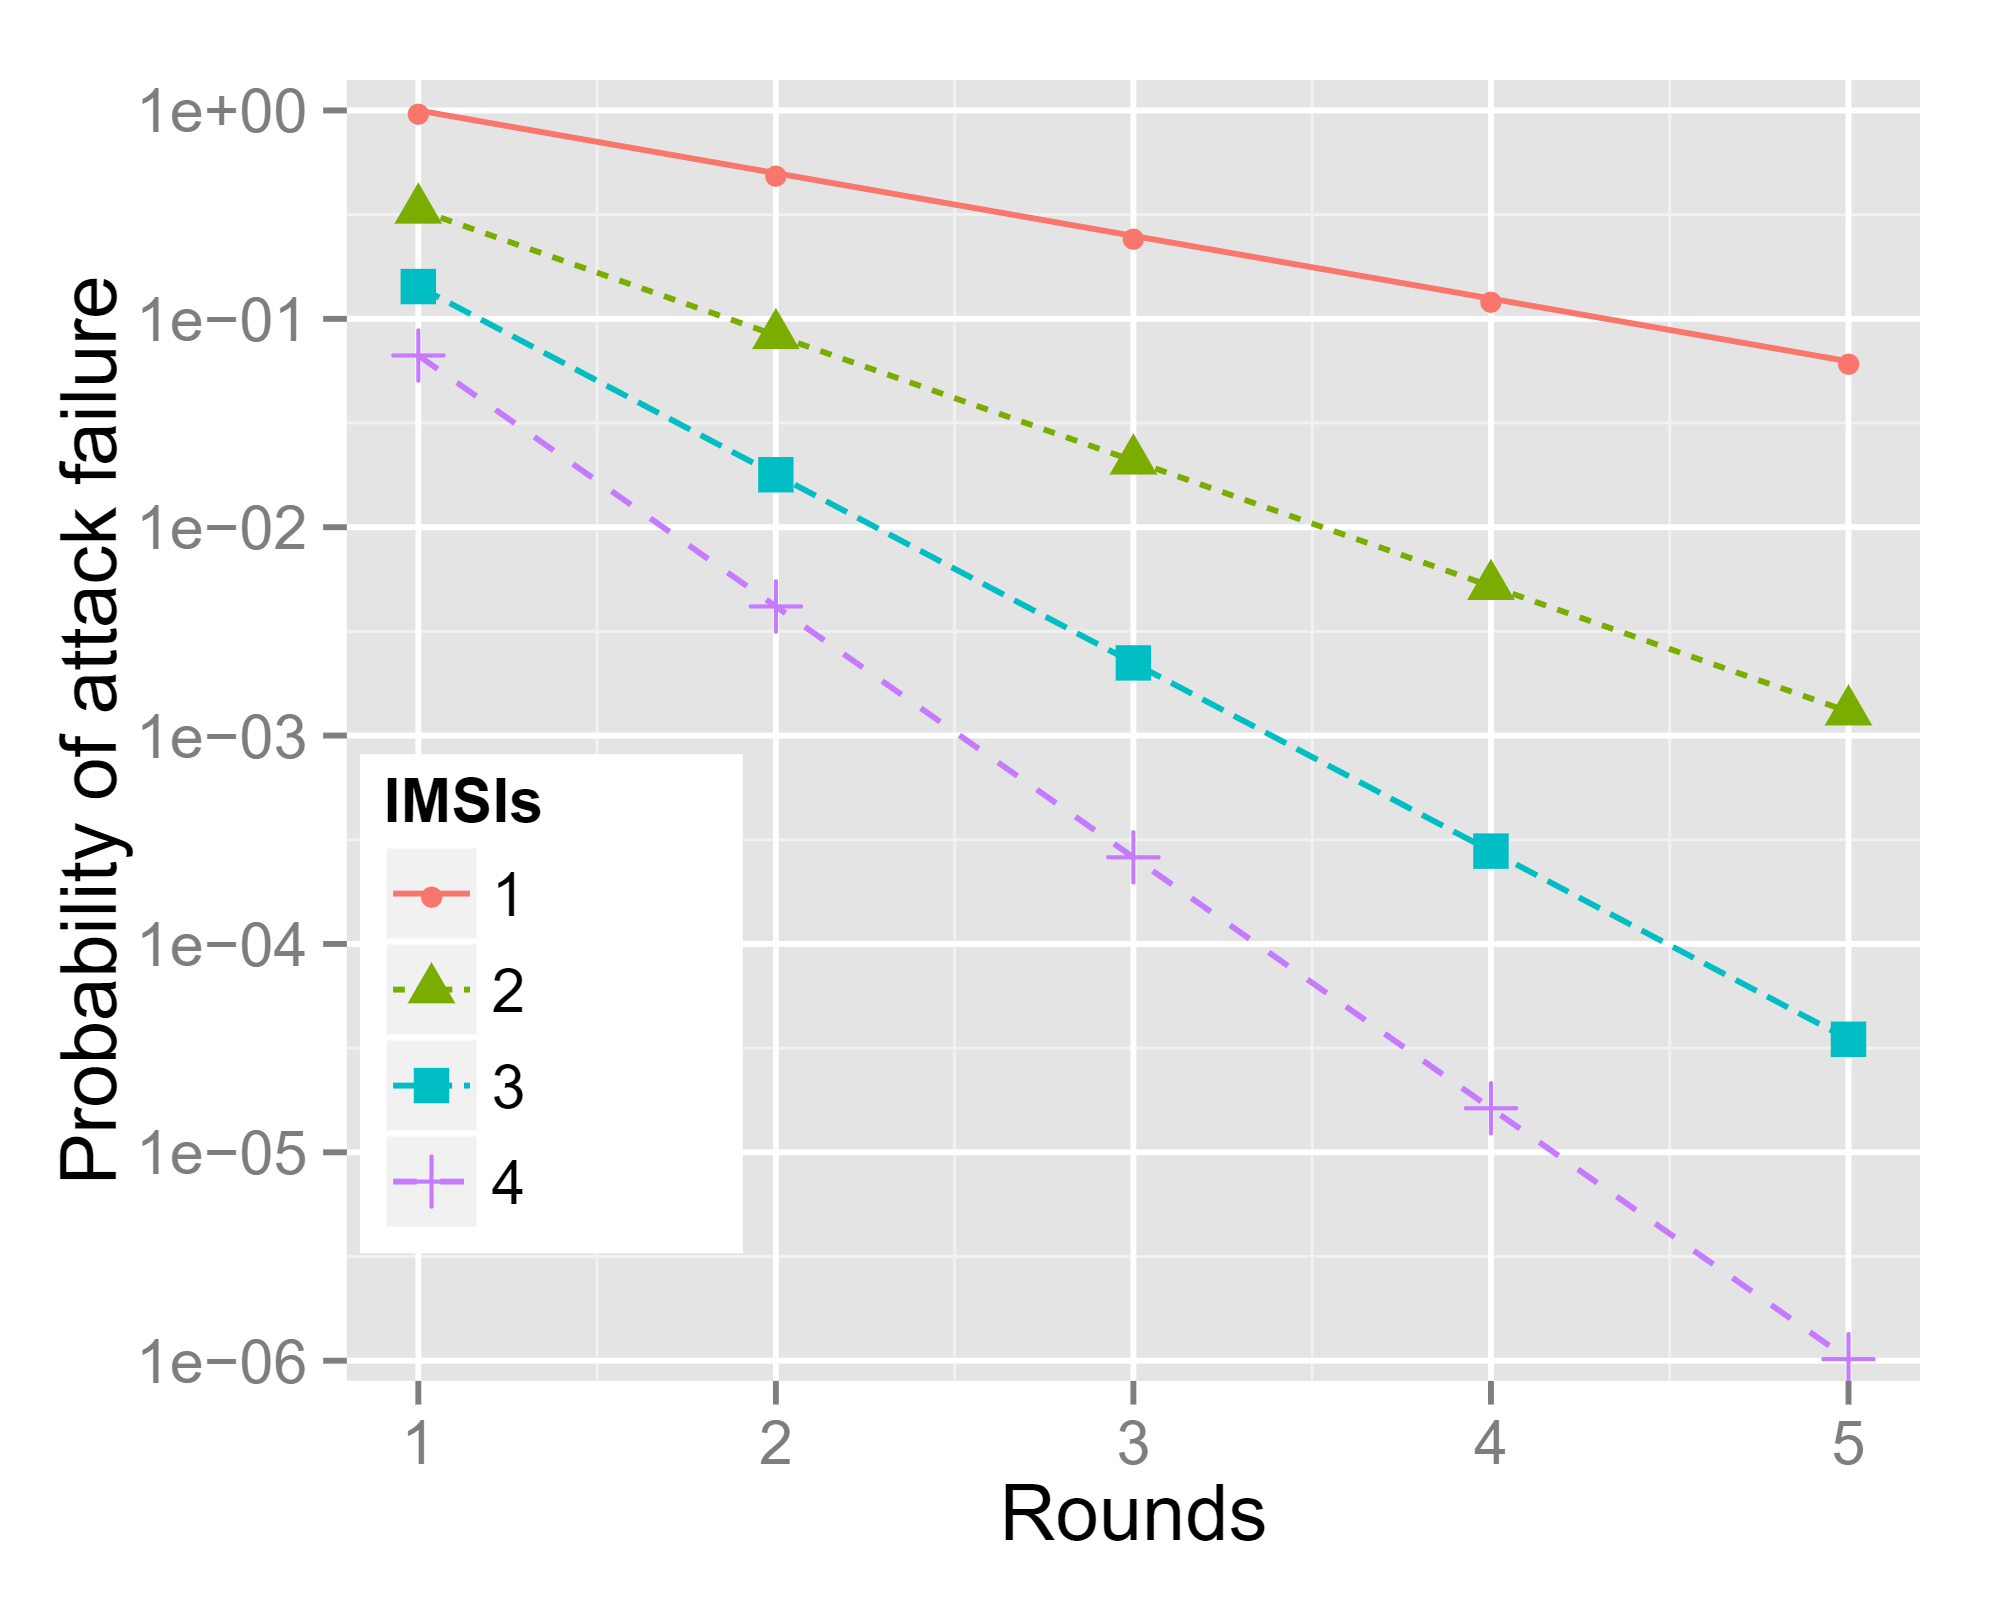
\includegraphics[width=.9\textwidth]{graphics/pageknock} }
	\caption{The probability that an attacker succeeds in crafting a fake page for varying  numbers of rounds $r$ and concurrent IMSIs $m$, based on Eq.~\ref{eq:pk}.}
	\label{fig:pk}
\end{figure}

A more efficient scheme where the phone registers $m$ IMSI values (one at a time)
from a single physical phone, all provided by the ZipPhone MVNO will take about 10--15 seconds to complete. Whenever the
proxy needs to contact the ZipPhone user, it selects a particular
non-empty, unordered subset of the $m$ values, and pages each IMSI
value in that order. Each IMSI can be paged once every 5.12 seconds with overlapping windows. 

For $m$ IMSI values, the number of non-empty unordered subsets for the first round is
$\sum_{i=2}^m{\binom{m}{i}}= 2^m-1.$ Because the empty subset can be included in subsequent rounds, 
for an 
$r$-round  sequence, the probability of the carrier guessing the
correct sequence  is
\begin{eqnarray}
\frac{1}{(2^m-1)(2^m)^{r-1}}. \label{eq:pk}
\end{eqnarray}
Figure~\ref{fig:pk} plots Eq.~\ref{eq:pk}. For example, when $m=3$ IMSIs are
used, the registration delay upon entering a new MSC region is 30--45
seconds. When $r=3$, the probability the carrier can guess the correct
sequence of pages is $0.002$. 

\section{Proposed work}

% TODO: simulate usability issues, simulate usage and trackability
% TODO: PRS and 
Some questions remain from the above work:
\begin{enumerate}
	\item How effective would location profiling and trajectory linking be in de-anonymizing ZipPhone or Spartacus users?
	\item How often would users need to go offline or significantly disrupt usage to avoid tracking?
\end{enumerate}

To answer these questions, I plan to simulate ZipPhone or Spartacus using data collected in Chapter~1. I will evaluate different de-anonymization algorithms, and different methods of evasion.

I will also try to implement Spartacus using SIMTrace hardware and simlabTrace\footnote{https://github.com/kamwar/simlabTrace/wiki}, which is able to sniff and perform a man-in-the-middle attack between the SIM card and phone. This would be a significant engineering effort to implement a modified handshake during the device's attach procedure to the network, and send information between devices.

%I plan to extend the location profiling analysis, as well as implement and evaluate a Spartacus implementation. This includes a trajectory linking algorithm to account for users who deftly try to avoid deanonymization by using different identities based on their location.
%
%\paragraph*{Spartacus implementation}
%To implement Sparatacus, one must perform a man-in-the-middle attack between SIM card and phone. I will investigate the use of SIMTrace and SIMLab to retrieve these credentials.
%
%In sum, I propose the following:
%\begin{enumerate}
%	\item Come up with a billing scheme
%	
%	\item Evaluate location privacy against some dataset or simulated dataset
%	
%	\item Evaluate pageknocking.
%	
%	\item Consider the cost to an attacker to deanonymize
%	
%	\item Investigate methods to estimate the size of a mix-zone.
%	
%	\item Model risk / utility of sharing your SIM with either someone you completely trust, or with a mix of peers that have a probability of turning against you.
%	
%	\item Implement an app that automatically shares an identity, goes dark, requests and identity.
%	
%	\item Implement Spartacus (PeerPhone)
%	
%	\item Test in the field. Evaluate performance and location inference with a mix-zone of 2 with the goal of finding out which new locations a user is visiting.
%	
%\end{enumerate}